\subsection{Relación 1}
\setcounter{ejercicio}{0}

\begin{ejercicio}\label{ej:1.1.1}
    Se considera el problema de encontrar las soluciones reales de la ecuación $x + \nicefrac{1}{2} - 2\sen(\pi x) = 0$ en el intervalo $\left[\nicefrac{1}{2},\nicefrac{3}{2}\right]$.
    \begin{enumerate}
        \item ¿Se puede utilizar el método de bisección para resolver dicho problema tomando $\left[\nicefrac{1}{2},\nicefrac{3}{2}\right]$ como intervalo inicial? ¿Por qué? En caso afirmativo, calcule las tres primeras iteraciones de dicho método.
        
        Definimos la función siguiente:
        \Func{f}{\left[\nicefrac{1}{2},\nicefrac{3}{2}\right]}{\bb{R}}{x}{x + \nicefrac{1}{2} - 2\sen(\pi x)}

        Sabemos que $f\in C^{\infty}\left(\left[\frac{1}{2},\frac{3}{2}\right]\right)$, y además:
        \begin{align*}
            f\left(\frac{1}{2}\right)&=1-2\sen\left(\frac{\pi}{2}\right)=-1<0\\
            f\left(\frac{3}{2}\right)&=2-2\sen\left(\frac{3\pi}{2}\right)=4>0
        \end{align*}

        Por lo tanto, por el teorema de Bolzano, existe al menos una raíz en el intervalo $\left[\nicefrac{1}{2},\nicefrac{3}{2}\right]$. Por tanto, podemos aplicar el método de bisección.
        Calculamos las tres primeras iteraciones:
        \begin{equation*}
            \begin{array}{c|cccc}
                n & a_n & b_n & x_n & f(x_n)\\
                \hline
                0 & 0.5 & 1.5 & 1 & 1.5\\
                1 & 0.5 & 1 & 0.75 & -0.1642\\
                2 & 0.75 & 1 & 0.875 & 0.6096\\
                3 & 0.75 & 0.875 & 0.8125
            \end{array}
        \end{equation*}
        \item Halle una cota del error que se comete si consideramos la última de las iteraciones del apartado anterior como el valor de la solución del problema dado.

        Tenemos que:
        \begin{equation*}
            |e_3| \leq \dfrac{1}{2^{4}}\left(\dfrac{3}{2}-\dfrac{1}{2}\right)=\dfrac{1}{16}=0.0625
        \end{equation*}
        \item ¿Cuántas iteraciones del método de bisección son necesarias para garantizar un error menor que $10^{-5}$?
        
        Para garantizar un error menor que $10^{-5}$ necesitamos que:
        \begin{align*}
            |e_n| \leq \dfrac{1}{2^{n+1}}\leq 10^{-5} \iff 10^5\leq 2^{n+1}\iff n\geq \log_2(10^5)-1\approx 15.6096
        \end{align*}

        Como $n$ debe ser entero, necesitamos al menos 16 iteraciones.
    \end{enumerate}
\end{ejercicio}

\begin{ejercicio}\label{ej:1.1.2}
    Se quiere calcular el inverso de un número real $c > 0$ sin efectuar divisiones. Para ello, se elige un valor $x_0 > 0$ y se considera el método iterativo dado por $x_{n+1} = x_n(2 - cx_n)$, $n \geq 0$.
    \begin{enumerate}
        \item Demuestre que la sucesión generada por dicho método converge a $\nicefrac{1}{c}$ si y sólo si $0 < x_0 < \nicefrac{2}{c}$.
        \begin{observacion}
            Comience demostrando por inducción que $r_n = r^{2^n}_0$ $\forall n \geq 0$ siendo $r_n = 1 - cx_n$.
        \end{observacion} 

        Demostramos por inducción dicha observación:
        \begin{itemize}
            \item \ul{Caso base}: $n=0$.
            \begin{equation*}
                r_0^{2^0}=r_0^1=r_0
            \end{equation*}

            \item \ul{Paso inductivo}: Supongamos que $r_n=r_0^{2^n}$.
            \begin{align*}
                r_0^{2^{n+1}}&=\left(r_0^{2^n}\right)^2=r_n^2=\left(1-cx_n\right)^2
                =1-2cx_n+c^2x_n^2
                = 1-cx_n\left(2-cx_n\right)
                =\\&= 1-cx_{n+1}=r_{n+1}
            \end{align*}

            Por lo tanto, $r_n=r_0^{2^n}$ para todo $n\geq 0$.
            Por la suma geométrica, tenemos que:
            \begin{align*}
                \{x_n\}\ \text{es convergente} &\iff \{r_n\}\ \text{es convergente} \iff\\&\iff |r_0|<1 \iff |1-cx_0|<1 \iff 0<cx_0<2\iff\\&\iff 0<x_0<\frac{2}{c}
            \end{align*}

            En el caso de que sea convergente, por la unicidad del límite, se tiene que:
            \begin{align*}
                1-c\lim_{n\to \infty}x_n
                =\lim_{n\to \infty} \left(1-cx_n\right)=
                \lim_{n\to \infty}r_n=0
                \Longrightarrow
                \lim_{n\to \infty}x_n = \frac{1}{c}
            \end{align*}
        \end{itemize}
        \item Demuestre que la convergencia referida en el apartado anterior es al menos cuadrática. ¿Cuál es la constante asintótica del error?
        
        Definimos la función siguiente:
        \Func{g}{\left[0,\frac{2}{c}\right]}{\bb{R}}{x}{x(2-cx)}

        Tenemos que:
        \begin{equation*}
            g\left(\frac{1}{c}\right)=\frac{1}{c}\left(2-\frac{c}{c}\right)=\frac{1}{c}
        \end{equation*}

        Calculamos las dos primeras derivadas de $g$:
        \begin{align*}
            g'(x)&=2-cx-cx=2(1-cx)\\
            g''(x)&=-2c
        \end{align*}

        Evaluando en el punto fijo de $g$:
        \begin{align*}
            g'\left(\frac{1}{c}\right)&=2(1-c\cdot\frac{1}{c})=2(1-1)=0\\
            g''\left(\frac{1}{c}\right)&=-2c\neq 0
        \end{align*}

        Por tanto, el método iterativo $x_{n+1}=g(x_n)$ tiene orden de convergencia cuadrático, con constante asintótica del error:
        \begin{equation*}
            C=\frac{1}{2}\cdot 2c=c
        \end{equation*}
        \item Compruebe que el método iterativo propuesto es el método de Newton-Raphson aplicado a una cierta ecuación $f(x) = 0$ cuya única raíz es $\nicefrac{1}{c}$.
        
        Sea $f$ la función que buscamos. Entonces:
        \begin{equation*}
            x-\dfrac{f(x)}{f'(x)} = g(x)=x(2-cx)
            \Longrightarrow
            \dfrac{f(x)}{f'(x)}=x-2x+cx^2=cx^2-x
        \end{equation*}

        Podríamos intentar resolver dicha ecuación diferencial en variables separadas, pero directamente probaremos con varias funciones que tienen a $\nicefrac{1}{c}$ como raíz, y veamos con cuál se da lo anterior.
        \begin{itemize}
            \item $f(x)=x-\nicefrac{1}{c}$.
            \begin{align*}
                f'(x)&=1\\
                \dfrac{f(x)}{f'(x)}&=f(x)=x-\nicefrac{1}{c}
            \end{align*}

            Por tanto, vemos que esta no es la función que buscamos.

            \item $f(x)=c-\nicefrac{1}{x}$.
            \begin{align*}
                f'(x)&=\nicefrac{1}{x^2}\\
                \dfrac{f(x)}{f'(x)}&=cx^2-x
            \end{align*}

            Por tanto, esta es la función que buscamos.
        \end{itemize}

        Por tanto, el método iterativo propuesto es el método de Newton-Raphson aplicado a la ecuación $f(x)=0$ con $f(x)=c-\nicefrac{1}{x}$, cuya única raíz es $\nicefrac{1}{c}$.
    \end{enumerate}
\end{ejercicio}


\begin{ejercicio}\label{ej:1.1.3}
    Demuestre que la ecuación $x^3 - 2x^2 - 5 = 0$ tiene una única solución en el intervalo $[1, 4]$. Elija una semilla $x_0$ que permita hallar, usando el método de Newton-Raphson, una aproximación a dicha solución y justifique dicha elección. Calcule las dos primeras iteraciones.

    Definimos la función siguiente:
    \Func{f}{[1,4]}{\bb{R}}{x}{x^3-2x^2-5}

    Sabemos que $f\in C^{\infty}([1,4])$, y además:
    \begin{align*}
        f(1)&=1-2-5=-6<0\\
        f(4)&=64-32-5=27>0
    \end{align*}

    Por lo tanto, por el teorema de Bolzano, existe al menos una raíz en el intervalo $[1,4]$. Veamos ahora que esta es única:
    \begin{equation*}
        f'(x)=3x^2-4x=x(3x-4)=0\iff x\in \left\{0,\frac{4}{3}\right\}
    \end{equation*}
    \begin{itemize}
        \item Si $x\in[1,\nicefrac{4}{3}]$, entonces $f'(x)\leq 0$.
        
        Como $f(1)<0$ y $f$ es continua, entonces $f$ no tiene raíces reales en $[1,\frac{4}{3}]$.
        \item Si $x\in[\nicefrac{4}{3},4]$, entonces $f'(x)\geq 0$.
        
        Como $f(\nicefrac{4}{3})<0$ y $f$ en este intervalo es inyectiva, entonces, de tener una raíz, sería única.
    \end{itemize}

    Por tanto, la ecuación $x^3-2x^2-5=0$ tiene una única solución en el intervalo $[\nicefrac{4}{3},4]$. Buscamos ahora demostrar la convergencia de Newton-Raphson:
    \begin{enumerate}
        \item $f(\nicefrac{4}{3})f(4)<0$.
        \item $f'(x)$ no se anula en $]\nicefrac{4}{3},4]$.
        \item $f''(x)=6x-4$ no se anula en $]\nicefrac{4}{3},4]$.
        \item Comprobemos que tomar $x_0=4$ sirve para garantizar la convergencia.
        \begin{equation*}
            f(4)f''(4)=27\cdot 20=540>0
        \end{equation*}
    \end{enumerate}

    Por tanto, podemos aplicar el método de Newton-Raphson empleando como semilla $x_0=4$. Calculamos las dos primeras iteraciones:
    \begin{equation*}
        \begin{array}{c|c}
            n & x_n\\
            \hline
            0 & 4\\
            1 & 3.15625\\
            2 & 2.77860
        \end{array}
    \end{equation*}
\end{ejercicio}


\begin{ejercicio}\label{ej:1.1.4}
    Deduzca la fórmula para el cálculo de las iteraciones del método de la secante a partir de su interpretación gráfica.

    Dados dos puntos $(x_n, f(x_n))$ y $(x_{n-1}, f(x_{n-1}))$, la recta secante que pasa por ellos es:
    \begin{equation*}
        \dfrac{y-f(x_{n})}{x-x_{n}}=\dfrac{f(x_n)-f(x_{n-1})}{x_n-x_{n-1}}
    \end{equation*}

    El punto de corte de la recta secante con el eje $x$ es:
    \begin{align*}
        \dfrac{0-f(x_{n})}{x-x_{n}}&=\dfrac{f(x_n)-f(x_{n-1})}{x_n-x_{n-1}}\\
        x-x_{n}&=-f(x_{n})\dfrac{x_n-x_{n-1}}{f(x_n)-f(x_{n-1})}\\
        x&=x_{n}-f(x_{n})\dfrac{x_n-x_{n-1}}{f(x_n)-f(x_{n-1})}
    \end{align*}

    Por tanto, denotamos por $x_{n+1}$ a dicho punto de corte, y obtenemos la fórmula del método de la secante:
    \begin{equation*}
        x_{n+1}=x_n-f(x_n)\dfrac{x_n-x_{n-1}}{f(x_n)-f(x_{n-1})}
    \end{equation*}
\end{ejercicio}


\begin{ejercicio}\label{ej:1.1.5}
    Dada la ecuación $x - \nicefrac{1}{2}\cos(x) = 0$, se pide:
    \begin{enumerate}
        \item Demuestre que tiene una única solución real en el intervalo $\left[0,\nicefrac{\pi}{2}\right]$.
        
        Definimos la función siguiente:
        \Func{f}{[0,\nicefrac{\pi}{2}]}{\bb{R}}{x}{x-\nicefrac{1}{2}\cos(x)}

        Sabemos que $f\in C^{\infty}([0,\nicefrac{\pi}{2}])$. Estudiemos su monotonía:
        \begin{align*}
            f'(x)=1+\nicefrac{1}{2}\sen(x)>0\ \forall x\in[0,\nicefrac{\pi}{2}]
        \end{align*}
        Por tanto, $f$ es inyectiva. Veamos ahora que tiene una única raíz:
        \begin{align*}
            f(0)&=0-\nicefrac{1}{2}\cos(0)=\nicefrac{-1}{2}<0\\
            f\left(\nicefrac{\pi}{2}\right)&=\nicefrac{\pi}{2}>0
        \end{align*}
        Por el teorema de Bolzano, existe al menos una raíz en el intervalo $[0,\nicefrac{\pi}{2}]$. Por la inyectividad de $f$, esta raíz es única.
        
        \item\label{ej:1.1.5b}
        Describa un método de iteración funcional, distinto del método de Newton-Raphson, que permita aproximar dicha solución, razonando la respuesta.\\

        Definimos la función siguiente:
        \Func{g}{[0,\nicefrac{\pi}{2}]}{\bb{R}}{x}{\nicefrac{1}{2}\cos(x)}

        Veamos que las raíces de $f$ son los puntos fijos de $g$:
        \begin{align*}
            f(x)=0&\iff x=\nicefrac{1}{2}\cos(x)\iff x=g(x)
        \end{align*}

        Comprobamos que la función será contractiva en un entorno del punto fijo $s$:
        \begin{equation*}
            |g'(x)|=\nicefrac{1}{2}|\sen(x)|\leq \nicefrac{1}{2}<1
        \end{equation*}

        Por tanto, podemos aplicar el método de iteración funcional $x_{n+1}=g(x_n)$ para aproximar la solución de la ecuación $x-\nicefrac{1}{2}\cos(x)=0$ partiendo de una semilla $x_0$ suficientemente próxima a la solución. Para especificar cuánto es ``suficientemente próxima'', veamos que $g\left([0,\nicefrac{\pi}{2}]\right)\subset [0,\nicefrac{\pi}{2}]$. Sea $x\in[0,\nicefrac{\pi}{2}]$, y entonces:
        \begin{equation*}
            0\leq g(x)=\frac{1}{2}\cos(x)\leq \frac{1}{2}<\frac{\pi}{2}
        \end{equation*}

        Por tanto, $g$ es una contracción en $[0,\nicefrac{\pi}{2}]$, y por tanto, podemos aplicar el método de iteración funcional para aproximar la solución de la ecuación $x-\nicefrac{1}{2}\cos(x)=0$.

        
        \item Realice las dos primeras iteraciones del método descrito en el apartado anterior.
        \begin{equation*}
            \begin{array}{c|c}
                n & x_n\\
                \hline
                0 & \nicefrac{\pi}{4}\approx 0.785398\\
                1 & 0.3535533\\
                2 & 0.4690742\\
                3 & 0.4459936
            \end{array}
        \end{equation*}
        \item ¿Cuántas iteraciones es preciso realizar para garantizar un error menor que $10^{-2}$ en el método dado en el apartado \ref{ej:1.1.5b}?
        
        Para garantizar un error menor que $10^{-2}$ necesitamos que:
        \begin{align*}
            |e_n|&\leq \dfrac{L^n}{1-L}\cdot |x_{1}-x_0|\leq \frac{1}{2^{n}(1-\nicefrac{1}{2})}\cdot |x_1-x_0|=\frac{0.43199}{2^{n-1}}
            \leq 10^{-2}\iff\\&\iff 2^{n-1}\geq \frac{0.43199}{10^{-2}}= 43.199
            \iff n\geq \log_2(43.199)+1\approx 6.4329
        \end{align*}

        Como $n$ debe ser entero, necesitamos al menos 7 iteraciones.
    \end{enumerate}
\end{ejercicio}

\begin{ejercicio}\label{ej:1.1.6}
    Usando algún resultado sobre convergencia para los métodos de iteración funcional, demuestre el teorema de convergencia local para ceros simples del método de Newton-Raphson.\\

    Sea $f$ una función de clase $C^2$ en un entorno de la raíz $s$ de la ecuación $f(x)=0$, y sea $f'(s)\neq 0$. Consideramos la función siguiente, definida en un entorno de $s$:
    \begin{equation*}
        g(x)=x-\frac{f(x)}{f'(x)}
    \end{equation*}

    Sabemos que $g(s)=s$. Calculemos su derivada:
    \begin{equation*}
        g'(x)=1-\frac{f'(x)f'(x)-f(x)f''(x)}{f'(x)^2}=\frac{f(x)f''(x)}{f'(x)^2}=0<1
    \end{equation*}

    Por tanto, por el Teorema de Convergencia Local de los métodos de iteración funcional, existe un intervalo que contiene a la raíz de forma que el método de Newton-Raphson converge a la raíz de forma cuadrática para cualquier semilla en dicho intervalo.
\end{ejercicio}

\begin{ejercicio}\label{ej:1.1.7}
    Para resolver la ecuación $f(x) = 0$ se considera el siguiente método, donde $m \neq 0$:
    $$x_{n+1} = x_n - \frac{f(x_n)}{m}$$
    \begin{enumerate}
        \item Interprete gráficamente el cálculo de las iteraciones según dicho método.
        
        Tenemos que:
        \begin{equation*}
            x_{n+1} = x_n - \frac{f(x_n)}{m}
            \Longrightarrow
            x_{n+1}-x_n  = \frac{-f(x_n)}{m}
            \Longrightarrow
            m = \frac{0-f(x_n)}{x_{n+1}-x_n}
        \end{equation*}

        Por tanto, pensando en la ecuación punto-pendiente de la recta, vemos que $x_{n+1}$ se calcula como el punto de corte de la recta que pasa por el punto $(x_n, f(x_n))$ y tiene pendiente $m$ con el eje $x$.
        \item ¿Qué condiciones para la función $f$, para la constante $m$ y para el valor inicial $x_0$ asegurarían unicidad de solución y convergencia a dicha solución del método considerado?

        Definimos la función siguiente:
        \Func{g}{I}{\bb{R}}{x}{x-\frac{f(x)}{m}}

        Debido a que no conocemos mucho sobre $f$, no podremos llegar a grandes resultados. Tan solo podremos garantizar resultados locales, por lo que usaremos el Teorema de la Convergencia Local. Consideramos $s\in I$ raíz de $f$, es decir, $f(s)=0$. Entonces, $g(s)=s$. Calculamos la derivada de $g$:
        \begin{equation*}
            g'(x)=1-\frac{f'(x)}{m}
        \end{equation*}

        Imponemos ahora $|g'(s)|<1$ para garantizar la convergencia local:
        \begin{equation*}
            |g'(s)|=\left|1-\frac{f'(s)}{m}\right|<1
            \iff 0<\frac{f'(s)}{m}<2
        \end{equation*}

        Por tanto, garantizando $0<\nicefrac{f'(s)}{m}<2$ se tiene que el método converge a la raíz $s$ de forma local; es decir, para semillas suficientemente cercanas a $s$.
    \end{enumerate}
\end{ejercicio}

\begin{ejercicio}\label{ej:1.1.8}
    Localice un intervalo $[a, b]$ en el que se encuentren todas las soluciones reales de la ecuación $2x^4 - 3x^2 + 3x - 4 = 0$, y sepárelas. Tomando $x_0 = -2$ como semilla, calcule las tres primeras iteraciones del método de Newton-Raphson usando el algoritmo de Horner.\\


    En primer lugar, calculamos:
    \begin{equation*}
        \alpha=\max\left\{\dfrac{2}{2}, \dfrac{3}{2}, \dfrac{3}{2}, \dfrac{4}{2}\right\}=2
    \end{equation*}

    Por tanto, tenemos que todas las raíces de la ecuación $2x^4-3x^2+3x-4=0$ están en el intervalo $[-3,3]$. Para separarlas, construimos la sucesión de Sturm correspondiente.
    Definimos:
    \polymul\ResAnt{2x^4-3x^2+3x-4}{1}
    \polymul\Res{8x^3-6x+3}{1}
    \begin{align*}
        f_0(x) &= p(x) = \polyprint\ResAnt\\
        f_1(x) &= f_0'(x) = \polyprint\Res
    \end{align*}

    Calculamos ahora $f_2(x)$.
    \begin{equation*}
        \polylongdiv[style=D]\ResAnt\Res
    \end{equation*}
    \polydiv\div\ResAnt\Res
    \polymul\ResAnt\Res{1}
    \polymul\Res\polyremainder{-4}

    Para simplificar, establecemos:
    \begin{align*}
        f_2(x) &= -4\cdot R(f_0(x), f_1(x))\\
        &= -4\cdot \left(\polyprint\polyremainder\right)\\
        &= \polyprint\Res
    \end{align*}

    Calculamos ahora $f_3(x)$.
    \begin{equation*}
        \polylongdiv[style=D]\ResAnt\Res
    \end{equation*}
    \polydiv\div\ResAnt\Res
    \polymul\ResAnt\Res{1}
    \polymul\Res\polyremainder{-3}

    Para simplificar, establecemos:
    \begin{align*}
        f_3(x) &= -3\cdot R(f_1(x), f_2(x))\\
        &= -3\cdot \left(\polyprint\polyremainder\right)\\
        &= \polyprint\Res
    \end{align*}

    Calculamos ahora $f_4(x)$.
    \begin{equation*}
        \polylongdiv[style=D]\ResAnt\Res
    \end{equation*}
    \polydiv\div\ResAnt\Res
    \polymul\ResAnt\Res{1}
    \polymul\Res\polyremainder{-392/39941}

    Para simplificar, establecemos:
    \begin{align*}
        f_4(x) &= -\dfrac{392}{39941}\cdot R(f_2(x), f_3(x))\\
        &= -\dfrac{392}{39941}\cdot \left(\polyprint\polyremainder\right)\\
        &= \polyprint\Res
    \end{align*}

    Por tanto, la sucesión de Sturm es:
    \begin{align*}
        f_0(x) &= 2x^4 - 3x^2 + 3x - 4\\
        f_1(x) &= 8x^3 - 6x + 3\\
        f_2(x) &= 6x^2-9x+16\\
        f_3(x) &= 28x+87\\
        f_4(x) &= -1
    \end{align*}

    Separamos ahora las raíces:
        \begin{equation*}
            \begin{array}{c|c|c|c|c|c|c}
                x & \sgn(f_0(x)) & \sgn(f_1(x)) & \sgn(f_2(x)) & \sgn(f_3(x)) & \sgn(f_4(x)) & \text{Nº Cambios Signo}\\ \hline
                -3& + & - & + & + & - & 3\\
                -2& + & - & + & + & - & 3\\
                -1& - & + & + & + & - & 2\\
                0 & - & + & + & + & - & 2\\
                1 & - & + & + & + & - & 2\\
                2 & + & + & + & + & - & 1\\
                3 & + & + & + & + & - & 1
            \end{array}
        \end{equation*}

    Por tanto, tenemos que hay una raíz en $[-2,-1]$ y otra en el intervalo $[1,2]$.
    Calculamos ahora las tres primeras iteraciones del método de Newton-Raphson con semilla $x_0=-2$ (aunque no hallamos demostrado la convergencia):
    \begin{equation*}
        \begin{array}{c|c|c|c}
            n & x_n & f(x_n) & f'(x_n)\\ \hline
            0 & -2 & 10 & -49\\
            1 & -1.795918 & 1.741690 & -32.563821\\
            2 & -1.742433 & 0.099956 & -28.866623\\
            3 & -1.738970
        \end{array}
    \end{equation*}
    donde tan solo se muestran las evaluaciones con Horner para $x_0$:
    \begin{equation*}
        \begin{array}{c|cccccc}
                & 2 & 0 & -3 & 3 & -4 \\
            -2 &   & -4 & 8 & -10 & 14\\          \hline
            & 2 & -4 & 5 & -7 & \boxed{10}\\
            -2 & & -4 & 16 & -42 \\ \hline
            & 2 & -8 & 21 & \boxed{-49} \\
        \end{array}
    \end{equation*}
\end{ejercicio}

\begin{ejercicio}\label{ej:1.1.9}
    Sea $s = \sqrt{3}$. Para calcular $s$ se considera el método de iteración funcional 
    \begin{equation*}
        x_{n+1} = g(x_n) \quad \text{con} \quad g(x) = \dfrac{ax + x^3}{3 + bx^2}.
    \end{equation*}

    Halle los valores de $a$ y $b$ para que, partiendo de una semilla $x_0$ suficientemente próxima a $s$, se asegure la convergencia al menos cuadrática. Para tales valores, calcule $x_3$ para $x_0 = 1$.\\

    En primer lugar, es necesario probar que $g(s)=s$ para que $s$ sea un punto fijo de $g$:
    \begin{equation*}
        s = g\left(s\right)=\dfrac{as+s^3}{3+bs^2} = \dfrac{as+3s}{3+3b}
        \Longrightarrow as+3s=3s+3bs
        \Longrightarrow a=3b
    \end{equation*}

    Por otro lado, para asegurar la convergencia local al menos cuadrática, es necesario que $g'(s)=0$:
    \begin{align*}
        g'(s)&=\dfrac{(a+3s^2)(3+bs^2)-(as+s^3)2bs}{(3+bs^2)^2}
        = \dfrac{(a+9)(3+3b)-(as+3s)2bs}{(3+3b)^2}=0\iff\\&\iff \begin{cases}
            3+3b\neq 0\\
            (a+9)(3+3b)-(as+3s)2bs=0
        \end{cases}
    \end{align*}

    Empleando que $a=3b$, obtenemos:
    \begin{equation*}
        (3b+9)(3+3b)-(3b+3)2bs^2=0
        \Longrightarrow (3+3b)(3b+9-6b)=0\Longrightarrow -3b+9=0\Longrightarrow b=3
    \end{equation*}

    Por tanto, $a=9,~b=3$. Calculamos ahora las tres primeras iteraciones con $x_0=1$ (aunque no hayamos demostrado la convergencia):
    \begin{equation*}
        \begin{array}{c|c}
            n & x_n\\ \hline
            0 & 1\\
            1 & 1.666667\\
            2 & 1.732026\\
            3 & 1.732051
        \end{array}
    \end{equation*}
\end{ejercicio}

\begin{ejercicio}\label{ej:1.1.10}
    Se desea aplicar un método iterativo del siguiente tipo para obtener $\sqrt[3]{7}$.
    $$x_{n+1} = p\cdot x_n + q\cdot \dfrac{7}{x^2_n} + r\cdot \dfrac{7^2}{x^5_n}$$
    Halle los valores de $p$, $q$, $r$ para que la convergencia local del método sea al menos cúbica. Realice dos iteraciones partiendo de $x_0 = 2$.\\

    Definimos la función siguiente:
    \Func{g}{\bb{R}^*}{\bb{R}}{x}{p\cdot x + q\cdot \dfrac{7}{x^2} + r\cdot \dfrac{49}{x^5}}

    Sea ahora $s=\sqrt[3]{7}$, de la cual tan solo conocemos que $s^3=7$. En primer lugar, es necesario probar que $s$ es un punto fijo de $g$:
    \begin{equation*}
        s = g\left(s\right)=p\cdot s + q\cdot \dfrac{7}{s^2} + r\cdot \dfrac{49}{s^5}
    \end{equation*}

    Dividiendo entre $s$ (que sabemos que es distinto de 0), obtenemos:
    \begin{equation*}
        1 = p + q\cdot \dfrac{7}{s^3} + r\cdot \dfrac{49}{s^6}
        \Longrightarrow 1 = p + q\cdot \dfrac{7}{7} + r\cdot \dfrac{49}{49}
        \Longrightarrow 1 = p + q + r
    \end{equation*}

    Por otro lado, para asegurar la convergencia local al menos cúbica, es necesario que $g'(s)=g''(s)=0$:
    \begin{align*}
        g'(s)&=p-\dfrac{7\cdot 2q}{s^3}-\dfrac{49\cdot 5r}{s^6}=0
        \Longrightarrow p-2q-5r=0\\
        g''(s)&=\dfrac{7\cdot 2\cdot 3q}{s^4}+\dfrac{49\cdot 5\cdot 6r}{s^7}=0
        \Longrightarrow \dfrac{6q}{s}+\dfrac{30r}{s}=0
        \Longrightarrow q+5r=0
    \end{align*}

    Por tanto, el sistema de ecuaciones a resolver es:
    \begin{equation*}
        \begin{cases}
            p+q+r=1\\
            p-2q-5r=0\\
            q+5r=0
        \end{cases}
    \end{equation*}

    De la tercera ecuación, obtenemos $q=-5r$, y sustituyendo en la segunda obtenemos $p=q$. sustituyendo en la primera ecuación, tenemos:
    \begin{equation*}
        -5r-5r+r=1\Longrightarrow -9r=1\Longrightarrow r=-\dfrac{1}{9}
        \Longrightarrow\begin{cases}
            p=\nicefrac{5}{9}\\
            q=\nicefrac{5}{9}\\
            r=\nicefrac{-1}{9}
        \end{cases}
    \end{equation*}

    Realizamos ahora las dos primeras iteraciones con $x_0=2$ (aunque no hayamos demostrado la convergencia):
    \begin{equation*}
        \begin{array}{c|c}
            n & x_n\\ \hline
            0 & 2\\
            1 & 1.9131944\\
            2 & 1.9129312
        \end{array}
    \end{equation*}
\end{ejercicio}

\begin{ejercicio}\label{ej:1.1.11}
    Sea $f(x) = x^5 + x^2 - 1$.
    \begin{enumerate}
        \item ¿Cuántas raíces tiene la ecuación $f(x) = 0$ en el intervalo $[0, 1]$?
        
        Podríamos demostrarlo estudiando la monotonía y haciendo uso del Teorema de Bolzano, pero de cara al último apartado lo haremos calculando la sucesión de Sturm.
        Definimos:
        \polymul\ResAnt{x^5+x^2-1}{1}
        \polymul\Res{5x^4+2x}{1}
        \begin{align*}
            f_0(x) &= p(x) = \polyprint\ResAnt\\
            f_1(x) &= f_0'(x) = \polyprint\Res
        \end{align*}

        Calculamos ahora $f_2(x)$.
        \begin{equation*}
            \polylongdiv[style=D]\ResAnt\Res
        \end{equation*}
        \polydiv\div\ResAnt\Res
        \polymul\ResAnt\Res{1}
        \polymul\Res\polyremainder{-5}

        Para simplificar, establecemos:
        \begin{align*}
            f_2(x) &= -5\cdot R(f_0(x), f_1(x))\\
            &= -5\cdot \left(\polyprint\polyremainder\right)\\
            &= \polyprint\Res
        \end{align*}

        Calculamos ahora $f_3(x)$.
        \begin{equation*}
            \polylongdiv[style=D]\ResAnt\Res
        \end{equation*}
        \polydiv\div\ResAnt\Res
        \polymul\ResAnt\Res{1}
        \polymul\Res\polyremainder{-9}

        Para simplificar, establecemos:
        \begin{align*}
            f_3(x) &= -9\cdot R(f_1(x), f_2(x))\\
            &= -9\cdot \left(\polyprint\polyremainder\right)\\
            &= \polyprint\Res
        \end{align*}

        Calculamos ahora $f_4(x)$.
        \begin{equation*}
            \polylongdiv[style=D]\ResAnt\Res
        \end{equation*}
        \polydiv\div\ResAnt\Res
        \polymul\ResAnt\Res{1}
        \polymul\Res\polyremainder{-108/15085}

        Para simplificar, establecemos:
        \begin{align*}
            f_4(x) &= -\dfrac{108}{15085}\cdot R(f_2(x), f_3(x))\\
            &= -\dfrac{108}{15085}\cdot \left(\polyprint\polyremainder\right)\\
            &= \polyprint\Res
        \end{align*}

        Por tanto, la sucesión de Sturm es:
        \begin{align*}
            f_0(x) &= x^5 + x^2 - 1\\
            f_1(x) &= 5x^4 + 2x\\
            f_2(x) &= -3x^2+5\\
            f_3(x) &= -18x-125\\
            f_4(x) &= 1
        \end{align*}

        Antes de separar las raíces, calculamos un intervalo en el cual estén todas las raíces. Para ello, calculamos:
        \begin{equation*}
            \alpha=\max\left\{1,1,1\right\}=1
        \end{equation*}

        Por tanto, tenemos que todas las raíces de la ecuación $x^5+x^2-1=0$ están en el intervalo $[-2,2]$. Separamos ahora las raíces:
        \begin{equation*}
            \begin{array}{c|c|c|c|c|c|c}
                x & \sgn(f_0(x)) & \sgn(f_1(x)) & \sgn(f_2(x)) & \sgn(f_3(x)) & \sgn(f_4(x)) & \text{Nº Cambios Signo}\\ \hline
                -2& - & + & - & - & + & 3\\
                -1& - & + & + & - & + & 3\\
                0 & - & 0 & + & - & + & 3\\
                1 & + & + & + & - & + & 2\\
                2 & + & + & - & - & + & 2
            \end{array}
        \end{equation*}
        Por tanto, tan solo tiene una raíz real, y está en el intervalo $[0,1]$.
        \item Pruebe que el método de iteración funcional
        $$x_{n+1} = g(x_n) = \sqrt{\dfrac{1}{x_n^3+1}}$$
        converge en el intervalo $[0, 1]$ a una raíz de $f(x) = 0$.\\

        Comprobemos en primer lugar que tiene puntos fijos. Tenemos que:
        \begin{equation*}
            g(x)=x\iff x=\sqrt{\dfrac{1}{x^3+1}}\iff x^2=\dfrac{1}{x^3+1}\iff x^5+x^2-1=0\iff f(x)=0
        \end{equation*}

        Por tanto, $g$ tiene como único punto fijo la raíz de $f$ en $[0,1]$.
        
        Comprobemos ahora que su primera derivada está acotada por uno. Calculémosla:
        \begin{align*}
            g'(x)&= \dfrac{\sqrt{x^3+1}}{2}\cdot \dfrac{-3x^2}{(x^3+1)^2}
            = -\dfrac{3}{2}\cdot \dfrac{x^2}{(x^3+1)^{\nicefrac{3}{2}}}\\
            g''(x)&=-\dfrac{3}{2}\cdot \dfrac{2x(x^3+1)^{\nicefrac{3}{2}}-x^2\cdot \nicefrac{3}{2}\cdot (x^3+1)^{\nicefrac{1}{2}}\cdot 3x^2}{(x^3+1)^3}
            =\\&=-\dfrac{3}{2}\cdot \dfrac{2x(x^3+1)-x^2\cdot \nicefrac{3}{2}\cdot 3x^2}{(x^3+1)^{\nicefrac{5}{2}}}
            =\\&=-\dfrac{12x(x^3+1)-x^2\cdot9\cdot 3x^2}{4(x^3+1)^{\nicefrac{5}{2}}}
            =-\dfrac{-15x^4+12x}{4(x^3+1)^{\nicefrac{5}{2}}}
            =\dfrac{3x(5x^3-4)}{4(x^3+1)^{\nicefrac{5}{2}}}
        \end{align*}

        Por tanto, los candidatos a extremos relativos de $g'$ son el $0$ y $\sqrt[3]{\nicefrac{4}{5}}$. Estudiamos la monotonía en $[0,1]$:
        \begin{itemize}
            \item Si $x\in [0,\sqrt[3]{\nicefrac{4}{5}}[$, entonces $g''(x)<0$.
            \item Si $x\in ]\sqrt[3]{\nicefrac{4}{5}},1]$, entonces $g''(x)>0$.
        \end{itemize}

        Evaluamos en el mínimo local y en los extremos del intervalo:
        \begin{align*}
            g'(0)&=0\\
            g'\left(\sqrt[3]{\nicefrac{4}{5}}\right)&=-\dfrac{3}{2}\cdot \dfrac{\sqrt[3]{\nicefrac{16}{25}}}{(\nicefrac{9}{5})^{\nicefrac{3}{2}}}
            = -\dfrac{\sqrt[6]{12500}}{9}\approx -0.53
            \\
            g'(1)&=-\dfrac{3}{2}\cdot \dfrac{1}{2\sqrt{2}}=-\dfrac{3}{4\sqrt{2}}\approx -0.53
        \end{align*}

        Por tanto, uniendo ambos resultados, para cada $x\in [0,1]$ se tiene que:
        \begin{equation*}
            -0.53\leq g'(x)\leq 0
            \Longrightarrow
            |g'(x)|<1
        \end{equation*}

        Por tanto, $g$ es contráctil. Notemos que no es necesario demostrar que $g\left([0,1]\right)\subseteq [0,1]$ ya que ya hemos demostrado la existencia y unicidad del punto fijo. Por tanto, por el Teorema de Convergencia de los Métodos de Iteración Funcional, el método de iteración funcional converge al punto fijo de $g$ en $[0,1]$, que es la raíz de $f$ en $[0,1]$.
        
        \item Localice todas las raíces reales de $f(x)$.
        
        Ya se ha realizado en el primer apartado.
    \end{enumerate}
\end{ejercicio}

\begin{ejercicio}\label{ej:1.1.12}
    A partir de la gráfica de $y = f(x)$ que se muestra, determine gráficamente las dos aproximaciones siguientes que generan los métodos de Newton-Raphson y de la secante partiendo de las semillas que aparecen en cada caso. Deduzca si hay convergencia y hacia qué solución de $f(x) = 0$.
    \begin{enumerate}
        \item Método de Newton-Raphson: El enunciado se muestra en la Figura~\ref{fig:1.12_1}, y la solución en la Figura~\ref{fig:1.12_1_sol}.
        
        Podemos intuir que el método de Newton-Raphson convergerá a la segunda raíz de $f$ comenzando por la izquierda.
        \item Método de la secante: El enunciado se muestra en la Figura~\ref{fig:1.12_2}, y la solución en la Figura~\ref{fig:1.12_2_sol}.
        
        Podemos intuir de nuevo que el método de la secante convergerá a la segunda raíz de $f$ comenzando por la izquierda.
    \end{enumerate}
\end{ejercicio}


\begin{figure}
    \centering
    \begin{tikzpicture}
        \begin{axis}[
            axis x line=center,
            axis y line=center,
            xmin=-1,
            xmax=1,
            ymin=-0.5,
            ymax=0.6,
            domain=-0.85:0.9,
            samples=100,
            % No haya ticks
            xtick=\empty,
            ytick=\empty,
        ]
            \addplot[blue, thick] {4*x^4 - 0.5*x^3 - 3*x^2 + 0.3};


            % 0.6, f(0.6)
            \addplot[mark=*] coordinates {(0.6335, -0.3868473793072)};

            % x_0 en el punto (0.6, 0)
            \addplot[mark=*] coordinates {(0.6335, 0)};
            \node[above] at (axis cs:0.6, 0) {$x_0$};

            % Recta dicontinua que une (0.6, 0) con (0.6, f(0.6))
            \addplot[dashed] coordinates {(0.6335, 0) (0.6335, -0.3868473793072)};
        \end{axis}
    \end{tikzpicture}
    \caption{Semilla para el método de Newton-Raphson en el Ejercicio \ref{ej:1.1.12}.}
    \label{fig:1.12_1}
\end{figure}

\begin{figure}
    \centering
    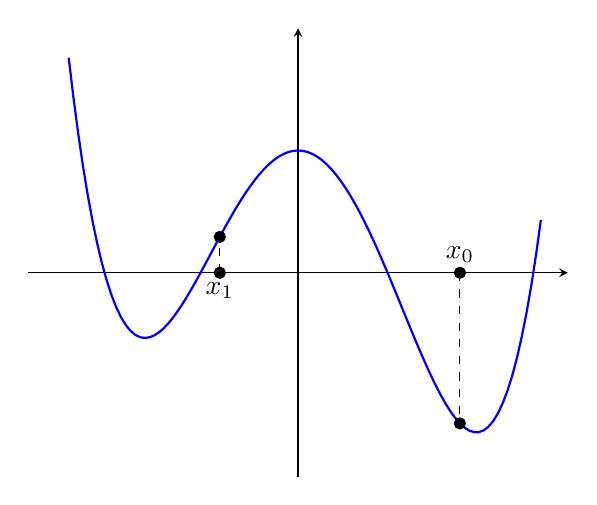
\begin{tikzpicture}
        \begin{axis}[
            axis x line=center,
            axis y line=center,
            xmin=-1,
            xmax=1,
            ymin=-0.5,
            ymax=0.6,
            domain=-0.85:0.9,
            samples=100,
            % No haya ticks
            xtick=\empty,
            ytick=\empty,
        ]
            \addplot[blue, thick] {4*x^4 - 0.5*x^3 - 3*x^2 + 0.3};


            % (0.6, -0.3696)
            \addplot[mark=*] coordinates {(0.6, -0.3696)};

            % x_0 en el punto (0.6, 0)
            \addplot[mark=*] coordinates {(0.6, 0)};
            \node[above] at (axis cs:0.6, 0) {$x_0$};

            % Recta dicontinua que une (0.6, 0) con (0.6, f(0.6))
            \addplot[dashed] coordinates {(0.6, 0) (0.6, -0.3696)};


            % (-0.29, 0.08818574)
            \addplot[mark=*] coordinates {(-0.29, 0.08818574)};

            % x_0 en el punto (-0.29, 0)
            \addplot[mark=*] coordinates {(-0.29, 0)};
            \node[below] at (axis cs:-0.29, 0) {$x_1$};

            % Recta dicontinua que une (-0.29, 0) con (-0.29, f(-0.29))
            \addplot[dashed] coordinates {(-0.29, 0) (-0.29, 0.08818574)};
        \end{axis}
    \end{tikzpicture}
    \caption{Semilla para el método de la Secante en el Ejercicio \ref{ej:1.1.12}.}
    \label{fig:1.12_2}
\end{figure}

\begin{figure}
    \centering
    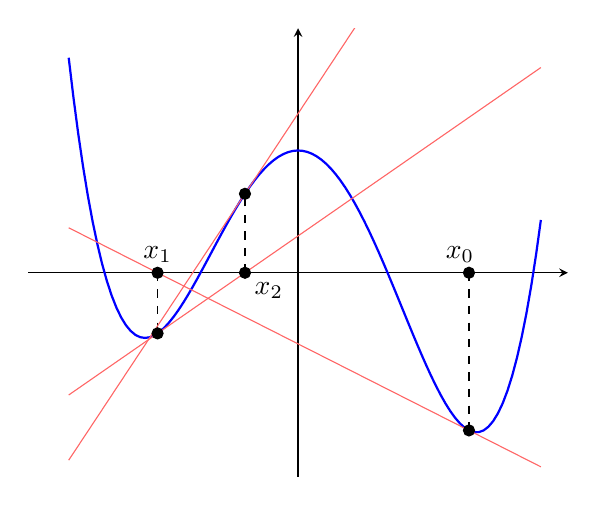
\begin{tikzpicture}
        \begin{axis}[
            axis x line=center,
            axis y line=center,
            xmin=-1,
            xmax=1,
            ymin=-0.5,
            ymax=0.6,
            domain=-0.85:0.9,
            samples=2,
            % No haya ticks
            xtick=\empty,
            ytick=\empty,
        ]
            \addplot[blue, thick, samples=100] {4*x^4 - 0.5*x^3 - 3*x^2 + 0.3};


            % 0.6, f(0.6)
            \addplot[mark=*] coordinates {(0.6335, -0.3868473793072)};

            % x_0 en el punto (0.6, 0)
            \addplot[mark=*] coordinates {(0.6335, 0)};
            \node[above] at (axis cs:0.6, 0) {$x_0$};

            % Recta dicontinua que une (0.6, 0) con (0.6, f(0.6))
            \addplot[dashed] coordinates {(0.6335, 0) (0.6335, -0.3868473793072)};

            % y = -0.335181049x - 0.1745101847657
            \addplot[red!60] {-0.335181049*x - 0.1745101847657};

            % X_1 Punto de Corte (-0.5206445450493, 0)
            \addplot[mark=*] coordinates {(-0.5206445450493, 0)};
            \node[above] at (axis cs:-0.5206445450493, 0) {$x_1$};

            % Imagen del Punto (-0.5206445450493, -0.1487290859193)
            \addplot[mark=*] coordinates {(-0.5206445450493, -0.1487290859193)};

            % Recta dicontinua que une (-0.5206445450493, 0) con (-0.5206445450493, -0.1487290859193)
            \addplot[dashed] coordinates {(-0.5206445450493, 0) (-0.5206445450493, -0.1487290859193)};

            % y = 0.4591571041328x + 0.0903285556681
            \addplot[red!60] {0.4591571041328*x + 0.0903285556681};

            % X_2 Punto de Corte (-0.1967269042667, 0)
            \addplot[mark=*] coordinates {(-0.1967269042667, 0)};
            \node[below right] at (axis cs:-0.1967269042667, 0) {$x_2$};

            % Imagen del Punto (-0.1967269042667, 0.1936936027091)
            \addplot[mark=*] coordinates {(-0.1967269042667, 0.1936936027091)};

            % Recta dicontinua que une (-0.1967269042667, 0) con (-0.1967269042667, 0.1936936027091)
            \addplot[dashed] coordinates {(-0.1967269042667, 0) (-0.1967269042667, 0.1936936027091)};

            % y = 1.000491271863x + 0.3905171533686
            \addplot[red!60] {1.000491271863*x + 0.3905171533686};
        \end{axis}
    \end{tikzpicture}
    \caption{Solución para el método de Newton-Raphson en el Ejercicio \ref{ej:1.1.12}.}
    \label{fig:1.12_1_sol}
\end{figure}






\begin{figure}
    \centering
    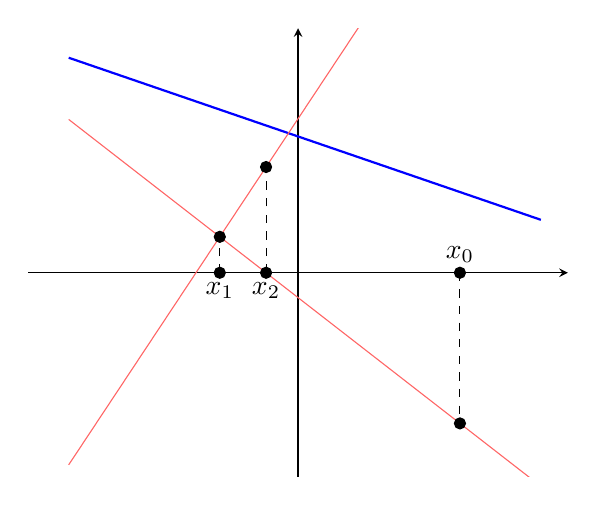
\begin{tikzpicture}
        \begin{axis}[
            axis x line=center,
            axis y line=center,
            xmin=-1,
            xmax=1,
            ymin=-0.5,
            ymax=0.6,
            domain=-0.85:0.9,
            samples=2,
            % No haya ticks
            xtick=\empty,
            ytick=\empty,
        ]
            \addplot[blue, thick, samples=2] {4*x^4 - 0.5*x^3 - 3*x^2 + 0.3};


            % (0.6, -0.3696)
            \addplot[mark=*] coordinates {(0.6, -0.3696)};

            % x_0 en el punto (0.6, 0)
            \addplot[mark=*] coordinates {(0.6, 0)};
            \node[above] at (axis cs:0.6, 0) {$x_0$};

            % Recta dicontinua que une (0.6, 0) con (0.6, f(0.6))
            \addplot[dashed] coordinates {(0.6, 0) (0.6, -0.3696)};


            % (-0.29, 0.08818574)
            \addplot[mark=*] coordinates {(-0.29, 0.08818574)};

            % x_0 en el punto (-0.29, 0)
            \addplot[mark=*] coordinates {(-0.29, 0)};
            \node[below] at (axis cs:-0.29, 0) {$x_1$};

            % Recta dicontinua que une (-0.29, 0) con (-0.29, f(-0.29))
            \addplot[dashed] coordinates {(-0.29, 0) (-0.29, 0.08818574)};

            % -0.45778574x - 0.89y = 0.054272556
            \addplot[red!60] {-0.45778574/0.89*x - 0.054272556/0.89};

            % X2 (-0.1185544923265, 0)
            \addplot[mark=*] coordinates {(-0.1185544923265, 0)};
            \node[below] at (axis cs:-0.1185544923265, 0) {$x_2$};

            % Imagen de X2 (-0.1185544923265, 0.2594578396311)
            \addplot[mark=*] coordinates {(-0.1185544923265, 0.2594578396311)};

            % Recta dicontinua que une (-0.1185544923265, 0) con (-0.1185544923265, 0.2594578396311)
            \addplot[dashed] coordinates {(-0.1185544923265, 0) (-0.1185544923265, 0.2594578396311)};

            % -0.1712720996311x + 0.1714455076735y = 0.0647879578569
            \addplot[red!60] {0.1712720996311/0.1714455076735*x + 0.0647879578569/0.1714455076735};

        \end{axis}
    \end{tikzpicture}
    \caption{Solución para el método de la Secante en el Ejercicio \ref{ej:1.1.12}.}
    \label{fig:1.12_2_sol}
\end{figure}


\begin{ejercicio}\label{ej:1.1.13}
    Se considera la ecuación $xe^{\nicefrac{-x}{3}} + 1 = 0$ y los métodos de iteración funcional $x_{n+1} = g(x_n)$ dados por las funciones
    \begin{align*}
        g_1(x) &= -e^{\nicefrac{x}{3}}, & g_2(x) &= e^{\nicefrac{x}{3}}, \\
        g_3(x) &= 3\ln(-x), & g_4(x) &= \dfrac{x-e^{\nicefrac{x}{3}}}{2}.
    \end{align*}
    \begin{enumerate}
        \item Encuentre un intervalo de amplitud 1 donde haya una única raíz de la ecuación.
        
        Definimos la siguiente función:
        \Func{f}{\bb{R}}{\bb{R}}{x}{xe^{\nicefrac{-x}{3}} + 1}

        Tenemos que $f\in C^1(\bb{R})$, y además:
        \begin{align*}
            f(0)&=1\\
            f(-1)&=-e^{\nicefrac{1}{3}}+1<0\iff e^{\nicefrac{1}{3}}>1\iff e>1
        \end{align*}

        Por tanto, la ecuación $xe^{\nicefrac{-x}{3}} + 1 = 0$ tiene una raíz en el intervalo $[-1,0]$. Veamos ahora si es la única en dicho intervalo.
        \begin{align*}
            f'(x)&=e^{\nicefrac{-x}{3}}-\dfrac{x}{3}e^{\nicefrac{-x}{3}}=e^{\nicefrac{-x}{3}}\left(1-\dfrac{x}{3}\right)=0\iff x=3
        \end{align*}

        Por tanto, como $f'$ no se anula en $[-1,0]$, entonces $f$ es inyectiva en $[-1,0]$, y por tanto la raíz en $[-1,0]$ es única.
        \item Averigüe cuáles de los métodos propuestos son compatibles con la ecuación dada; es decir, para cuáles de ellos la solución es punto fijo.
        \begin{align*}
            g_1(x)&=x\iff -e^{\nicefrac{x}{3}}=x\iff -e^{\nicefrac{x}{3}-\nicefrac{x}{3}}=xe^{\nicefrac{-x}{3}}\iff -e^0=xe^{\nicefrac{-x}{3}}\iff\\&\iff xe^{\nicefrac{-x}{3}}+1=0\iff f(x)=0\\
            g_2(x)&=x\iff e^{\nicefrac{x}{3}}=x\Longrightarrow x>0\Longrightarrow x\notin [-1,0]\Longrightarrow g_2\text{ no es compatible}\\
            g_3(x)&=x\iff 3\ln(-x)=x\iff \ln(-x)=\nicefrac{x}{3}\iff \ln(1)-\ln(-x)=-\nicefrac{x}{3}\iff\\&\iff \ln\left(\nicefrac{1}{-x}\right)=\nicefrac{-x}{3}\iff \nicefrac{1}{-x}=e^{\nicefrac{-x}{3}}\iff xe^{-\nicefrac{x}{3}}+1=0\iff f(x)=0\\
            g_4(x)&=x\iff \dfrac{x-e^{\nicefrac{x}{3}}}{2}=x\iff x-e^{\nicefrac{x}{3}}=2x\iff -e^{\nicefrac{x}{3}}=x\iff\\&\iff -1=xe^{\nicefrac{-x}{3}}\iff f(x)=0
        \end{align*}

        Por tanto, vemos que $g_1, g_3$ y $g_4$ son compatibles con la ecuación dada, mientras que $g_2$ no lo es.
        \item De entre los métodos compatibles con la ecuación ¿cuáles son convergentes localmente? Justifique la respuesta.
        
        Sea $s$ una raíz de $f$. Ya hemos visto que $s$ será un punto de fijo de $g_i$ para $i\in\{1,3,4\}$. Para estudiar la convergencia local, necesitamos acotar la primera derivada en un entorno de $s$, y como desconocemos el valor de $s$, hemos de acotarla en todo el intervalo $[-1,0]$.
        \begin{itemize}
            \item \ul{Para $g_1$}:
            \begin{align*}
                |g_1'(x)|=\dfrac{1}{3}e^{\nicefrac{x}{3}}\leq \dfrac{1}{3}e^{\nicefrac{0}{3}}=\dfrac{1}{3}<1\qquad \forall x\in [-1,0]
            \end{align*}
            Por tanto, $g_1$ es convergente localmente.

            \item \ul{Para $g_3$}:
            \begin{align*}
                |g_3'(x)|=\dfrac{3}{|x|}\geq 3>1\qquad \forall x\in [-1,0]
            \end{align*}
            Por tanto, $g_3$ no es convergente para ningún $x\in [-1,0]$.

            \item \ul{Para $g_4$}:
            \begin{align*}
                |g_4'(x)|=\dfrac{1}{2}\left|1-\dfrac{1}{3}e^{\nicefrac{x}{3}}\right|\leq \dfrac{1}{2}\left(1+\dfrac{1}{3}e^{\nicefrac{x}{3}}\right)\leq\dfrac{1}{2}\left(1+\dfrac{1}{3}\right)=\dfrac{2}{3}<1\qquad \forall x\in [-1,0]
            \end{align*}
            Por tanto, $g_4$ es convergente localmente.
        \end{itemize}
        \item De entre los métodos convergentes localmente ¿cuál es el más rápido? ¿Por qué?
        
        En primer lugar, estudiamos si la primera derivada se anula o no. Sabemos que:
        \begin{align*}
            g_1'(x)&=-\dfrac{1}{3}e^{\nicefrac{x}{3}}\neq 0\qquad \forall x\in [-1,0]\\
            g_4'(x)&=\dfrac{1}{2}\left(1-\dfrac{1}{3}e^{\nicefrac{x}{3}}\right)=0\iff e^{\nicefrac{x}{3}}=3\iff x=3\ln(3)\notin [-1,0]
        \end{align*}

        Por tanto, vemos que ambos tienen orden de convergencia lineal. Por tanto, para comparar cuál de ellos es más rápido, hemos de estudiar el valor de la constante asintótica del error. Notemos por $C_1$ y $C_4$ las constantes asintóticas de $g_1$ y $g_4$ respectivamente, y sea $s$ la raíz de $f$ en $[-1,0]$. Entonces, sabemos que:
        \begin{align*}
            C_1 = |g_1'(s)| = \dfrac{1}{3}e^{\nicefrac{s}{3}}\qquad C_4 = g_4'(s) = \dfrac{1}{2}\left|1-\dfrac{1}{3}e^{\nicefrac{s}{3}}\right|= \dfrac{1}{2}\left(1-\dfrac{1}{3}e^{\nicefrac{s}{3}}\right)
        \end{align*} 

        Comparémoslas:
        \begin{align*}
            C_1\leq C_4\iff \dfrac{1}{3}e^{\nicefrac{s}{3}}\leq \dfrac{1}{2}\left(1-\dfrac{1}{3}e^{\nicefrac{s}{3}}\right)\iff \dfrac{1}{2}e^{\nicefrac{s}{3}}\leq \dfrac{1}{2}\iff e^{\nicefrac{s}{3}}\leq 1\iff s\leq 0
        \end{align*}
        Como $s\in [-1,0]$, entonces $C_1\leq C_4$. Por tanto, como a menor constante asintótica, mayor velocidad de convergencia, entonces $g_1$ es más rápido que $g_4$.
        \item Para el método con mayor velocidad, aplique Steffensen con semilla $x_0 = -0.5$ hasta que dos iteraciones consecutivas disten menos de $10^{-3}$.
        
        Desarrollamos en primer lugar la aceleración de Aitken. Fijado $n\in \bb{N}$, tenemos que:
        \begin{align*}
            \Delta x_n &= x_{n+1}-x_n\\
            \Delta^2 x_n &= \Delta \Delta x_n = \Delta x_{n+1}-\Delta x_n = x_{n+2}-2x_{n+1}+x_n
        \end{align*}

        Por tanto, la aceleración de Aitken es:
        \begin{equation*}
            x_{n}^* = x_n - \dfrac{(\Delta x_n)^2}{\Delta^2 x_n}
        \end{equation*}

        Por tanto, aplicamos Steffensen a $g_1$ con semilla $x_0=-0.5$:
        \begin{equation*}
            \begin{array}{c|c|c|c}
                g_1 & \Delta x_n & \Delta^2 x_n & \text{Steffensen}\\ \hline
                -0.5 &&\\
                -0.846482&&\\
                -0.754152 & -0.346482 & 0.438811 & -0.773579\\
                -0.773579&&\\
                -0.772703&&\\
                -0.772929 & 0.000876 & -0.001101 & -0.772883\\
                -0.772883&&\\
                -0.772883&&\\
                -0.772883 & \approx 0 & \approx 0 & -0.772883                
            \end{array}
        \end{equation*}
    \end{enumerate}
\end{ejercicio}


\begin{ejercicio}\label{ej:1.1.14}
    Supongamos que se modifica el método de bisección cambiando el punto de división del intervalo por el valor $a + \frac{b-a}{3}$ (porque se cree que la solución está más cerca del extremo $a$). ¿Es convergente dicho método? ¿Cuál es la cota del error absoluto después de $n$ iteraciones?\\

    Sea $a_n$ la sucesión de extremos izquierdos de los intervalos en la $n$-ésima iteración, y sea $b_n$ la sucesión de extremos derechos de los intervalos en la $n$-ésima iteración. Entonces, por el Teorema de Bolzano aplicado a cada intervalo, tenemos que:
    \begin{align*}
        \exists s\in [a,b]\text{ tal que } s\in [a_n,b_n],\ f(s)=0\qquad \forall n\in \bb{N}
    \end{align*}

    Definimos ahora la sucesión de longitudes de los intervalos $l_n=b_n-a_n$. Calculamos ahora la longitud de los intervalos en la $n+1$-ésima iteración. Fijado el punto de disión $m_n=a_n+\dfrac{b_n-a_n}{3}$, caben dos posibilidades, quedarnos con el intervalo $[a_n,m_n]$ o con el intervalo $[m_n,b_n]$.
    \begin{itemize}
        \item Si optamos por el intervalo $[a_n,m_n]$, entonces:
        \begin{align*}
            a_{n+1}&=a_n\\
            b_{n+1}&=m_n=a_n+\dfrac{b_n-a_n}{3}
            l_{n+1}&=b_{n+1}-a_{n+1}=\dfrac{b_n-a_n}{3} = \dfrac{l_n}{3}
        \end{align*}

        \item Si optamos por el intervalo $[m_n,b_n]$, entonces:
        \begin{align*}
            a_{n+1}&=m_n=a_n+\dfrac{b_n-a_n}{3}\\
            b_{n+1}&=b_n\\
            l_{n+1}&=b_{n+1}-a_{n+1}=\dfrac{3b_n-3a_n-b_n+a_n}{3}=\dfrac{2b_n-2a_n}{3}=\dfrac{2l_n}{3}
        \end{align*}
    \end{itemize}
    
    
    En cualquier caso, tenemos que:
    \begin{align*}
        0\leq l_{n+1}\leq \max\left\{\dfrac{l_n}{3},\dfrac{2l_n}{3}\right\}=\dfrac{2}{3}l_n\leq \left(\dfrac{2}{3}\right)^2 l_{n-1}\leq \ldots \leq \left(\dfrac{2}{3}\right)^{n+1} l_0=\left(\dfrac{2}{3}\right)^{n+1}(b-a)
    \end{align*}

    Tomando límite cuando $n\to\infty$, por el Lema del Sandwich, tenemos que:
    \begin{equation*}
        \{a_n-b_n\}=\{l_n\}\to 0
    \end{equation*}

    La sucesión $\{a_n\}$ es creciente y acotada superiormente por $b$, y la sucesión $\{b_n\}$ es decreciente y acotada inferiormente por $a$. Por tanto, ambas sucesiones son convergentes, digamos que $a_n\to a^*$ y $b_n\to b^*$. Por tanto, por la unicidad del límite, tenemos que:
    \begin{equation*}
        0 = \lim_{n\to\infty}(l_n) = \lim_{n\to\infty}(b_n-a_n)=b^*-a^*
        \Longrightarrow a^*=b^*
    \end{equation*}
    Por tanto, ambas sucesiones convergen al mismo límite, llamémosle $L$. Además, previamente hemos visto que $\exists s\in [a,b]$, con $f(s)=0$, tal que:
    \begin{equation*}
        a_n\leq s\leq b_n\quad \forall n\in \bb{N}
    \end{equation*}

    Tomando límite cuando $n\to\infty$, por el Teorema del Sandwich, tenemos que $L=s$. Por tanto, veamos que la sucesión formada por este método converge a $s$:
    \begin{equation*}
        \{m_n\}=\left\{a_n+\dfrac{b_n-a_n}{3}\right\}\to s+\dfrac{s-s}{3}=s
    \end{equation*}

    Por tanto, el método es convergente. Por otro lado, la cota del error absoluto después de $n$ iteraciones es:
    \begin{equation*}
        |e_n|=|s-m_n|\leq l_{n+1}\leq \left(\dfrac{2}{3}\right)^{n+1}(b-a)
    \end{equation*}

    En conclusión, el método es convergente, y la cota del error absoluto después de $n$ iteraciones es mayor que la del método de bisección original, por lo que no hay garantías algunas de que sea preferible este método al original.
\end{ejercicio}

\begin{ejercicio}\label{ej:1.1.15}
    Demuestre el teorema de convergencia global de los métodos de iteración funcional para sistemas.
    \begin{observacion}
        Generalice al caso $k$-dimensional la demostración del teorema de convergencia global de los métodos de iteración funcional unidimensional.
    \end{observacion}
    \begin{enumerate}
        \item El primer paso se tiene de forma directa por el Teorema del Punto Fijo de Banach, que ya se demostró en Análisis Matemático II para $\bb{R}^n$.
        
        \item Sea $S$ el punto fijo de $G$. Tenemos que:
        \begin{equation*}
            \|X_n-S\|=\|G(X_{n-1})-G(S)\|\leq L\|X_{n-1}-S\|\leq \ldots \leq L^n\|X_0-S\|
            \qquad \forall n\in \bb{N}
        \end{equation*}

        Tomando límite cuando $n\to\infty$, tenemos que:
        \begin{equation*}
            \lim_{n\to\infty}\|X_n-S\|=0\Longrightarrow \{X_n\}\to S
        \end{equation*}

        Por tanto, el método es convergente.

        \item Busquemos ahora una cota del error. Necesitamos para ello eliminar la dependencia de $S$ de la cota anterior. Tenemos que:
        \begin{align*}
            \|X_0-S\| &= \|X_0-X_1+X_1-S\|\leq \|X_0-X_1\|+\|X_1-S\| \leq \|X_0-X_1\|+L\|X_0-S\|
        \end{align*}

        Despejando $\|X_0-S\|$:
        \begin{align*}
            \|X_0-S\| &\leq \|X_0-X_1\|+L\|X_0-S\|\\
            (1-L)\|X_0-S\| &\leq \|X_0-X_1\|\\
            \|X_0-S\| &\leq \dfrac{1}{1-L}\|X_0-X_1\|
        \end{align*}

        Por tanto, la cota del error es:
        \begin{equation*}
            \|E_n\|=\|X_n-S\|\leq \dfrac{L^n}{1-L}\|X_0-X_1\|
        \end{equation*}
    \end{enumerate}
\end{ejercicio}

\begin{ejercicio}\label{ej:1.1.16}
    Sea $D = \prod\limits_{i=1}^k[a_i, b_i]$ y sea $G : D \to \bb{R}^k$ con $G = (g_1, \ldots, g_k)$ tal que $G \in C^1(D)$. Demuestre que si existe $L \in\left]0, 1\right[$ tal que $\forall i, j = 1, \ldots, k$ se verifique
    \begin{equation*}
        \left\lvert \dfrac{\partial g_i(x)}{\partial x_j} \right\rvert \leq \dfrac{L}{k}\quad \forall x \in D,
    \end{equation*}
    entonces $G$ es contráctil.
    \begin{observacion}
        Considere la norma $\| \cdot \|_1$ o $\| \cdot \|_\infty$.
    \end{observacion}

    Para cada $x\in G$, consideramos $JG(x)$, que es la matriz jacobiana de $G$ en $x$. Calculamos su norma $1$, que es el máximo de las sumas de los valores absolutos de las columnas de $JG(x)$:
    \begin{align*}
        \|JG(x)\|_1 &= \max_{j=1,\ldots,k}\left\{\sum_{i=1}^k\left|\dfrac{\partial g_i(x)}{\partial x_j}\right|\right\}\leq \max_{j=1,\ldots,k}\left\{\sum_{i=1}^k\dfrac{L}{k}\right\}=\max_{j=1,\ldots,k}\left\{L\right\}=L
    \end{align*}

    Por tanto, por el Teorema del Valor Medio en $\bb{R}^k$, tenemos que:
    \begin{equation*}
        \|G(x)-G(y)\| \leq L\|x-y\|\quad \forall x,y\in D
    \end{equation*}

    Por tanto, $G$ es contráctil, con constante de Lipschitz $L<1$.
\end{ejercicio}

\begin{ejercicio}\label{ej:1.1.17}
    Se considera el sistema de ecuaciones
    \begin{align*}
        \dfrac{x^2-y^2}{2}-x + \frac{7}{24} &= 0, \\
        xy - y + \frac{1}{9} &= 0.
    \end{align*}
    \begin{enumerate}
        \item Demuestre que tiene una única solución en el rectángulo $D = [0, 0.4] \times [0, 0.4]$.
        
        Definimos las siguientes funciones:
        \Func{g_1}{D}{\bb{R}}{(x,y)}{\dfrac{x^2-y^2}{2} + \dfrac{7}{24}}
        \Func{g_2}{D}{\bb{R}}{(x,y)}{xy + \dfrac{1}{9}}

        Veamos en primer lugar que $g_1(D)\subset [0,0.4]$. Sean $x,y\in [0,0.4]$. Entonces:
        \begin{align*}
            0.21\approx -\dfrac{0.4^2}{2}+\dfrac{7}{24}\leq g_1(x,y)=\dfrac{x^2-y^2}{2}+\dfrac{7}{24}\leq \dfrac{0.4^2}{2}+\dfrac{7}{24}\approx 0.37
        \end{align*}

        Por tanto, $g_1(D)\subset [0,0.4]$. Veamos ahora que $g_2(D)\subset [0,0.4]$. Sean de nuevo $x,y\in [0,0.4]$. Entonces:
        \begin{align*}
            \dfrac{1}{9}\leq g_2(x,y)=xy+\dfrac{1}{9}\leq 0.4\cdot 0.4+\dfrac{1}{9}\approx 0.271
        \end{align*}

        Por tanto, $g_2(D)\subset [0,0.4]$. Definimos ahora $G=(g_1,g_2)$. Tenemos por tanto que $G:D\to D$. Veamos ahora que $G$ es contráctil. Para ello, calculamos la matriz jacobiana de $G$:
        \begin{align*}
            JG(x,y)=\begin{pmatrix}
                \dfrac{\partial g_1}{\partial x}(x,y) & \dfrac{\partial g_1}{\partial y}(x,y)\\
                \dfrac{\partial g_2}{\partial x}(x,y) & \dfrac{\partial g_2}{\partial y}(x,y)
            \end{pmatrix}=\begin{pmatrix}
                x & -y\\
                y & x
            \end{pmatrix}
        \end{align*}

        Calculamos ahora la norma de esta matriz:
        \begin{align*}
            \|JG(x,y)\|_1=\max\left\{|x|+|-y|,|y|+|x|\right\}=\max\{x+y,y+x\}=x+y\leq 2\cdot 0.4=0.8
        \end{align*}

        Por tanto, $G$ es contráctil, con constante de Lipschitz $L=0.8<1$. Por tanto, por el Teorema del Punto Fijo de Banach, $G$ tiene un único punto fijo en $D$. Además, sabemos que $X\in D$ es un punto fijo de $G$ si y solo si $X$ es solución del sistema de ecuaciones. Por tanto, el sistema de ecuaciones tiene una única solución en $D$.


        \item Encuentre una sucesión que converja a dicha solución, justificando la respuesta.
        
        Por el Teorema de Convergencia Global de los Métodos de Iteración Funcional para Sistemas, sabemos que el siguiente método es convergente al punto fijo de $G$ para cualquier semilla $X_0\in D$:
        \begin{equation*}
            X_{n+1}=G(X_n)\qquad \forall n\in \bb{N}
        \end{equation*}

        En forma matricial, tenemos que:
        \begin{equation*}
            \begin{pmatrix}
                x_{n+1}\\
                y_{n+1}
            \end{pmatrix}=\begin{pmatrix}
                \dfrac{x_n^2-y_n^2}{2}+\dfrac{7}{24}\\
                x_ny_n+\nicefrac{1}{9}
            \end{pmatrix}\qquad \forall n\in \bb{N}
        \end{equation*}

        Aunque no lo piden, calculamos las dos primeras iteraciones del método iterativo para la semilla $X_0=(0.1,0.2)$:
        \begin{equation*}
            \begin{array}{c|c|c}
                n & x_n & y_n\\ \hline
                0 & 0.1 & 0.2\\
                1 & 0.276667 & 0.131111\\
                2 & 0.321344 & 0.147385\\
                3 & 0.332436 & 0.158472
            \end{array}
        \end{equation*}
        \item Calcule, tomando $x_0 = (0.1, 0.2)$, las dos primeras iteraciones del método de Newton-Raphson para el sistema.
        
        Definimos las siguientes funciones:
        \Func{f_1}{\bb{R}^2}{\bb{R}}{(x,y)}{\dfrac{x^2-y^2}{2}-x+\dfrac{7}{24}}
        \Func{f_2}{\bb{R}^2}{\bb{R}}{(x,y)}{xy-y+\dfrac{1}{9}}

        Calculamos ahora la matriz jacobiana de $F=(f_1,f_2)$:
        \begin{align*}
            JF(x,y)=\begin{pmatrix}
                \dfrac{\partial f_1}{\partial x}(x,y) & \dfrac{\partial f_1}{\partial y}(x,y)\\
                \dfrac{\partial f_2}{\partial x}(x,y) & \dfrac{\partial f_2}{\partial y}(x,y)
            \end{pmatrix}=\begin{pmatrix}
                x-1 & -y\\
                y & x-1
            \end{pmatrix}
        \end{align*}

        Calculamos ahora el jacobiano de $f$ en punto arbitrario $(x,y)\in D$:
        \begin{equation*}
            |JF(x,y)|=(x-1)^2+y^2>0\qquad \forall (x,y)\in D
        \end{equation*}

        Por tanto, $\exists JF(x,y)^{-1}$, y por tanto, el método de Newton-Raphson es aplicable. Este es:
        \begin{align*}
            X_{n+1}&=X_n-JF(X_n)^{-1}F(X_n)
        \end{align*}

        Para resolverlo, tenemos dos opciones:
        \begin{description}
            \item[Opción 1] Calcular la inversa de $JF(x,y)$.
            
            Tenemos que:
            \begin{align*}
                JF(x,y)^{-1}=\dfrac{1}{(x-1)^2+y^2}\begin{pmatrix}
                    x-1 & y\\
                    -y & x-1
                \end{pmatrix}
            \end{align*}

            Por tanto, en forma matricial, el método de Newton-Raphson es:
            \begin{align*}
                \begin{pmatrix}
                    x_{n+1}\\
                    y_{n+1}
                \end{pmatrix}=\begin{pmatrix}
                    x_n\\
                    y_n
                \end{pmatrix}-\dfrac{1}{(x_n-1)^2+y_n^2}\begin{pmatrix}
                    x_n-1 & y_n\\
                    -y_n & x_n-1
                \end{pmatrix}\begin{pmatrix}
                    \dfrac{x_n^2-y_n^2}{2}-x_n+\dfrac{7}{24}\\
                    x_ny_n-y_n+\dfrac{1}{9}
                \end{pmatrix}
            \end{align*}

            Como vemos, los cálculos no son directos, puesto que hay que realizar diversas multiplicaciones de matrices a la hora de evaluar. No obstante, son cálculos sencillos. El resultado es:
            \begin{equation*}
                \begin{array}{c|c|c}
                    n & x_n & y_n\\ \hline
                    0 & 0.1 & 0.2\\
                    1 & 0.30327 & 0.16863\\
                    2 & 0.3327 & 0.1666\\
                    3 & 0.33333 & 0.166667
                \end{array}
            \end{equation*}

            \item[Opción 2] Sin necesidad de calcular la inversa de $JF(x,y)$.
            
            En este caso, el método de Newton-Raphson es:
            \begin{align*}
                X_{n+1} &= X_n-JF(X_n)^{-1}F(X_n)\\
                \Delta X_n &= -JF(X_n)^{-1}F(X_n)\\
                JF(X_n)\Delta X_n &= -F(X_n)
            \end{align*}

            En cada paso, calcularemos $\Delta X_n$ resolviendo dicho sistema de ecuaciones, y así podremos obtener posteriormente $X_{n+1}$. Los cálculos son igualmente tediosos, pero siguen sin ser tediosos. De esta forma, sí es cierto que nos ahorramos el cálculo de la inversa de $JF(x,y)$, pero a cambio, hemos de resolver un sistema de ecuaciones en cada paso. El resultado es el mismo que en la Opción 1.
        \end{description}
    \end{enumerate}
\end{ejercicio}


\begin{ejercicio}\label{ej:1.1.18}
    Se considera el sistema de ecuaciones
    \begin{align*}
        x - xy &= \nicefrac{1}{16}, \\
        x^2 - y &= \nicefrac{-1}{8}.
    \end{align*}
    \begin{enumerate}
        \item Demuestre que tiene una única solución en el rectángulo $D = [0, \nicefrac{1}{8}] \times [0, \nicefrac{1}{4}]$.
        
        Definimos las siguientes funciones:
        \Func{g_1}{D}{\bb{R}}{(x,y)}{xy+\nicefrac{1}{16}}
        \Func{g_2}{D}{\bb{R}}{(x,y)}{x^2+\nicefrac{1}{8}}

        Veamos en primer lugar que $g_1(D)\subset [0,\nicefrac{1}{8}]$. Sean $x\in [0,\nicefrac{1}{8}]$ e $y\in [0,\nicefrac{1}{4}]$. Entonces:
        \begin{align*}
            0\leq g_1(x,y)=xy+\frac{1}{16}\leq \frac{1}{8}\cdot\frac{1}{4}+\frac{1}{16}=\frac{1}{32}+\frac{1}{16}=\frac{3}{32}<\frac{4}{32}=\frac{1}{8}
        \end{align*}

        Por tanto, $g_1(D)\subset [0,\nicefrac{1}{8}]$. Veamos ahora que $g_2(D)\subset [0,\nicefrac{1}{4}]$. Sean de nuevo $x\in [0,\nicefrac{1}{8}]$ e $y\in [0,\nicefrac{1}{4}]$. Entonces:
        \begin{align*}
            0\leq g_2(x,y)=x^2+\frac{1}{8}\leq \frac{1}{8}^2+\frac{1}{8}=\frac{1}{64}+\frac{1}{8}=\frac{9}{64}<\frac{16}{64}=\frac{1}{4}
        \end{align*}

        Por tanto, $g_2(D)\subset [0,\nicefrac{1}{4}]$. Definimos ahora $G=(g_1,g_2)$. Tenemos por tanto que $G:D\to D$. Veamos ahora que $G$ es contráctil. Para ello, calculamos la matriz jacobiana de $G$:
        \begin{align*}
            JG(x,y)=\begin{pmatrix}
                \dfrac{\partial g_1}{\partial x}(x,y) & \dfrac{\partial g_1}{\partial y}(x,y)\\
                \dfrac{\partial g_2}{\partial x}(x,y) & \dfrac{\partial g_2}{\partial y}(x,y)
            \end{pmatrix}=\begin{pmatrix}
                y & x\\
                2x & 0
            \end{pmatrix}
        \end{align*}

        Calculamos ahora la norma de esta matriz:
        \begin{align*}
            \|JG(x,y)\|_1=\max\left\{|y|+|x|,|2x|\right\}=\max\{x+y,2x\}\leq \max\left\{\frac{1}{8}+\frac{1}{4},\frac{1}{4}\right\}=\frac{3}{8}<1
        \end{align*}

        Por tanto, $G$ es contráctil, con constante de Lipschitz $L=\nicefrac{3}{8}<1$. Por tanto, por el Teorema del Punto Fijo de Banach, $G$ tiene un único punto fijo en $D$. Además, sabemos que $X\in D$ es un punto fijo de $G$ si y solo si $X$ es solución del sistema de ecuaciones. Por tanto, el sistema de ecuaciones tiene una única solución en $D$.
        \item Encuentre una sucesión que converja a dicha solución, justificando la respuesta.
        
        Por el Teorema de Convergencia Global de los Métodos de Iteración Funcional para Sistemas, sabemos que el siguiente método es convergente al punto fijo de $G$ para cualquier semilla $X_0\in D$:
        \begin{equation*}
            X_{n+1}=G(X_n)\qquad \forall n\in \bb{N}
        \end{equation*}
        \item Calcule, tomando $x_0 = (0.1, 0.2)$, las dos primeras iteraciones del método de Newton-Raphson para el sistema.
        
        Definimos las siguientes funciones:
        \Func{f_1}{\bb{R}^2}{\bb{R}}{(x,y)}{x-xy-\nicefrac{1}{16}}
        \Func{f_2}{\bb{R}^2}{\bb{R}}{(x,y)}{x^2-y+\nicefrac{1}{8}}

        Calculamos ahora la matriz jacobiana de $F=(f_1,f_2)$:
        \begin{align*}
            JF(x,y)=\begin{pmatrix}
                \dfrac{\partial f_1}{\partial x}(x,y) & \dfrac{\partial f_1}{\partial y}(x,y)\\
                \dfrac{\partial f_2}{\partial x}(x,y) & \dfrac{\partial f_2}{\partial y}(x,y)
            \end{pmatrix}=\begin{pmatrix}
                1-y & -x\\
                2x & -1
            \end{pmatrix}
        \end{align*}

        Calculamos ahora el jacobiano de $f$ en punto arbitrario $(x,y)\in D$:
        \begin{equation*}
            |JF(x,y)|=(y-1)+2x^2\leq \left(\frac{1}{4}-1\right)+2\left(\frac{1}{8}\right)^2=-\frac{3}{4}+\frac{1}{32}=-\frac{24}{32}+\frac{1}{32}=-\frac{23}{32}<0
        \end{equation*}

        Por tanto, $\exists JF(x,y)^{-1}$, y por tanto, el método de Newton-Raphson es aplicable.
        Este es:
        \begin{align*}
            X_{n+1}&=X_n-JF(X_n)^{-1}F(X_n)
        \end{align*}

        Para resolverlo, optamos por la primera opción, calculando la inversa de $JF(x,y)$:
        \begin{align*}
            JF(x,y)^{-1}=\dfrac{1}{(y-1)+2x^2}\begin{pmatrix}
                -1 & x\\
                -2x & 1-y
            \end{pmatrix}
        \end{align*}

        Por tanto, en forma matricial, el método de Newton-Raphson es:
        \begin{align*}
            \begin{pmatrix}
                x_{n+1}\\
                y_{n+1}
            \end{pmatrix}=\begin{pmatrix}
                x_n\\
                y_n
            \end{pmatrix}-\dfrac{1}{(y_n-1)+2x_n^2}\begin{pmatrix}
                1-y_n & -x_n\\
                2x_n & -1
            \end{pmatrix}\begin{pmatrix}
                x_n-xy_n-\nicefrac{1}{16}\\
                x_n^2-y_n+\nicefrac{1}{8}
            \end{pmatrix}
        \end{align*}

        Como vemos, los cálculos no son directos, puesto que hay que realizar diversas multiplicaciones de matrices a la hora de evaluar. No obstante, son cálculos sencillos. El resultado es:
        \begin{equation*}
            \begin{array}{c|c|c}
                n & x_n & y_n\\ \hline
                0 & 0.1 & 0.2\\
                1 & 0.06923076923077 & 0.12884615384615\\
                2 & 0.07184796591410 & 0.13015528048751\\
                3 & 0.07185252471221 & 0.13016278528674
            \end{array}
        \end{equation*}

    \end{enumerate}
\end{ejercicio}